
\chapter{Case Study} \label{case_study}

The aim of this chapter is to present a more elaborate case study, using real data from the host group, providing a meaningful pipeline with the ability to demonstrate the application's features, as well as the ones of the underlying \textit{specmine} package. This case study consists in the chemometric characterization of the carotenoid content in cassava roots tissue, using \gls{uv}, CIELAB data and a \acrfull{llf} of the two.

Unlike the previous ones, the author was involved in this study since the beginning, being one of the authors of the respective publication, accepted and presented at the 11$^{th}$ International Conference on \gls{pacbb} during the development of this thesis \citep{moresco2017classification}. The extended version of the published study is in submission phase for the \textit{Journal of Inorganic Biochemistry} and is presented below.


\section{Introduction}

Cassava is the commonly used term to designate the \textit{Manihot esculenta} species. This tuberous-root plant species offers a wide variety of agronomic advantages, being resilient to droughts, inexpensive, resistant to major diseases and pests, easy to grow and having flexible harvest times, allowing farmers to harvest the roots as needed. It is, therefore, a valuable source of energy for people living in the poorest regions. However, cassava roots are a poor source of provitamin A carotenoids, whose deficiency is a major problem in such regions \citep{la2013biofortified, sanchez2014prediction}. 

Carotenoids are one of the most important natural pigments, having already been recognized benefits of carotenoid consumption, such as the diminished risk of several degenerative disorders, including various types of cancer, cardiovascular or ophthalmological diseases, as well as their preventive effect associated with their antioxidant activity, protecting cells and tissues from oxidative damage \citep{stahl2003antioxidant}. However, only vitamin A precursors $\beta$-carotene, $\alpha$-carotene and $\beta$-cryptoxanthin represent the major sources of carotenoids in the human diet.

With a broad range of colors, varying from yellow to dark-red, carotenoids confer color to many plant leaves, fruits and flowers, as well as birds, insects, fish, and crustaceans. The color of cassava's starchy root, which can vary from white to red, is strongly correlated to the presence and contents of several carotenoid pigments and their associations \citep{sanchez2006reduction}. However, the possibility of adopting the color of roots as an indirect criterion for selection of higher carotene content is questionable, since color is a characteristic of difficult visual evaluation. Thus, the use of a standardized color measurement technique is of most importance.

The CIELAB color technique was adopted by the \gls{cie} and is based on the Lab color space, which describes mathematically all perceivable colors in three dimensions: L* for lightness and a* and b* for the color opponents green-red and blue-yellow. The values of these three variables are usually absolute, with the L* value representing the darkest black at L* = 0, and the brightest white at L* = 100. On the other hand, the a* value represents red and green opponents at positive and negative values, respectively, while the b* value represents yellow and blue opponents at positive and negative values, respectively \citep{brockes1982evaluation, schanda2007colorimetry}. A visual representation of the CIELAB color space is shown in \autoref{cielab}.

\begin{figure}[h]
	\centering
	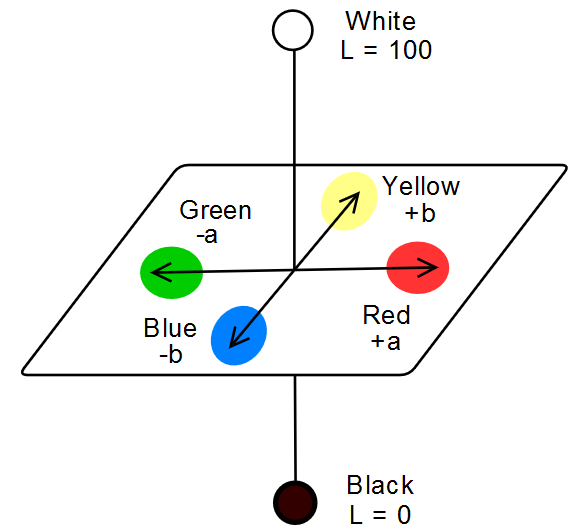
\includegraphics[width=0.4\linewidth]{Imagens/Case_study/cielab}
	\caption{Representation of the CIE L* a* b* color space.}
	\label{cielab}
\end{figure}

Currently, CIELAB is the most used system for quantitative color description of an object, given its uniformity, ease of acquisition, very low cost and device independence. Considering that this technique facilitates the acquisition of measurements directly on the field, while also avoiding the degradation of the compounds, it becomes an appealing approach in comparison to traditionally used methods such as \gls{hplc} or \gls{uv}. The CIELAB color technique has been applied for instance in the unique identification of skin color for clinical and scientific purposes \citep{weatherall1992skin} and as an optimal color design approach for transforming patients' perception into color elements \citep{liu2014optimal}.

Combining \gls{uv} and CIELAB colorimetric data, the aim of the present case study is to validate a quantification method for carotenoid content estimation in roots of \textit{M. esculenta}, assuming that the statistical and machine learning techniques can correlate these data types, to ultimately detect genotypes of \textit{M. esculenta} with high contents of carotenoids. Importantly, this study provides tools that can support the plant-breeding program at Epagri (Agricultural Research Company and Rural Extension of the State of Santa Catarina, \href{http://www.epagri.sc.gov.br/}{\nolinkurl{http://www.epagri.sc.gov.br/}}) that aims to obtain genotypes with high levels of pro-vitamin A carotenoids and superior nutritional traits.


\section{Materials and Methods} \label{MM}

\subsection{Selection of cassava genotypes} \label{cassava_gen}

Fifty root samples of \textit{M. esculenta} genotypes harvested in 2015/2016 season from the Epagri's germplasm bank (Urussanga Experimental Station, 28$^{\circ}$31'18''S, 49$^{\circ}$19'03''W, Santa Catarina, southern Brazil) were used in this study due to their economic and social importance.

All genotypes were cultivated under the same soil, climatic conditions and agricultural treatments. Importantly, the investigated genotypes were pre-selected according to their relevance for biofortification projects, due to the presence of carotenoids with provitamin A activity and lycopene (visual selection), low levels of cyanogenic glycosides and suitable agronomic traits (e.g., high yield, resistance to drought and to pests and diseases), being widely cultivated in southern Brazil. The fifty genotypes from the germplasm bank were, in fact, indicated by the Epagri plant breeder team given the samples' preference by local small farmers for commercial production due to their physiochemical variability.  


\subsection{Carotenoid extraction and quantification} \label{carot_quant}

Carotenoids were extracted from fresh cassava roots as described in  \cite{rodriguez2004harvestplus} using an Ultra-Turrax (Janke \& Kunkel IKA - T25 basic) and mixture of acetone: petroleum ether (v/v) as extraction solution.

The absorbances of the organosolvent extracts were then recorded on an \gls{uv} spectrophotometer (Gold Spectrum lab 53 \gls{uv} spectrophotometer, BEL photonics, Brazil) using a spectral window from 200 to 700 $\eta m$. Aliquots (10 $\mu l$) of the extracts were also injected into a liquid chromatograph (LC-10A Shimadzu) system equipped with a C18 reversed-phase column (Vydac 201TP54, 250$mm$ x 4.6$mm$, 5$\mu m$ $\phi$, 35$^{\circ}$C) coupled to a pre-column (C18 Vydac 201TP54, 30$mm$ x 4.6$mm$, 5$\mu m$ $\phi$) and a spectrophotometric detector (450 nm). A mixture of methanol: acetonitrile (90:10, v/v) was used for elution at a flow rate of 1 $mL$/min. The identification and quantification of compounds of interest was carried out via co-chromatography and comparison of retention times of samples with those of standard compounds (Sigma–Aldrich, USA) under the same experimental conditions.

The color measurements of the root samples were made immediately after harvest  using a colorimeter (CR-400, Minolta\textsuperscript{\tiny\textregistered}, Japan) and the results expressed according to the CIELAB color space scale \citep{la2013biofortified}. Three readings were performed at different sites for all fifty samples.


\subsection{Statistical Analysis} \label{stat}

Data relating to the quantification of carotenoids were expressed as the mean ($\mu g$ carotenoids $/g$ root - dry weight) $\pm$ standard deviation and submitted to an \gls{anova} followed by post-hoc Tukey's \gls{hsd} test (p $ < $ 0.05) for mean comparison.

Spectrophotometric data and the amounts of the target carotenoids determined by \gls{hplc} were treated using multivariate statistical analysis and chemometrics techniques supported by scripts written in R language (v. 3.3.1) (\href{https://cran.r-project.org/}{\nolinkurl{https://cran.r-project.org/}}).

All data analysis were supported and structured using the R \textit{specmine} package \citep{costa2016r}, developed within our research group. More information about the package and its features is available in \autoref{specmine_chapter}.


\subsection{Machine Learning} \label{ML}

To obtain machine learning models capable of accurately predicting the carotenoid contents in cassava roots, regression-derived statistical and machine learning models were used, such as \acrfull{lasso}, ridge and linear regression, regression trees, random forests, elastic network, \acrfull{pls}, \acrfull{svm}, and K-nearest neighbors models \citep{singh2007review, domingos2012few}. More information regarding machine learning is available in \autoref{supervised}.

Data from \gls{uv} spectrophotometry, CIELAB, as well as a fusion of the two were used as inputs to each of the referred machine learning models. Three response variables were used in the machine learning approach: the \gls{tcc} determined by spectrophotometry (Lambert-Beer law), the \gls{tcc} and the content of trans-$\beta$-carotene, the most abundant carotene in cassava roots, both determined by \gls{hplc}. A comprehensive scheme of the entire machine learning approach applied in the study is shown in \autoref{ml_diagram}.

\begin{figure}[h]
	\centering
	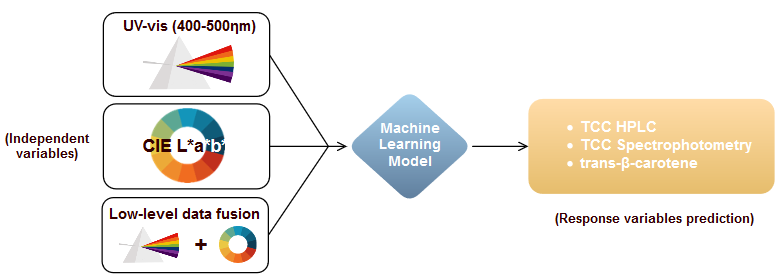
\includegraphics[width=1\linewidth]{Imagens/Case_study/ml_diagram}
	\caption{Machine learning approach used. Three different datasets were used as input to the models, namely the \gls{uv}, CIELAB and fusion datasets. The response variables used for prediction were the \gls{tcc} determined by spectrophotometry (Lambert-Beer law) and the \gls{tcc} and trans-$\beta$-carotene content determined by \gls{hplc}.}
	\label{ml_diagram}
\end{figure}

This being a regression problem, the chosen evaluation metrics to compare model performance were the \acrfull{rmse} and the coefficient of determination (R$^{2}$), since they explicitly show how much the model predictions deviate, on average, from the actual values in the dataset.


\subsubsection{UV-visible dataset}

Considering that most carotenoids exhibit absorption in the visible region of the spectrum, between 400 to 500 $\eta m$, a subset of the original \gls{uv} dataset was used, with samples belonging to this wavelength interval (101 features). Additionally, missing values contained within this dataset were replaced with the mean of the variables' values. 

Using the different response variables for prediction, the models that showed best performance were selected and the variable importance calculated. A set of pre-processing methods was applied to the datasets to see whether model performance could be improved, using the models that showed best performance with raw data. These pre-processing methods included smoothing interpolation, scaling, \acrfull{msc}, first derivative calculation and background, offset and baseline corrections. The data was also subject to filter-based feature selection (40\%, 60\% and 80\% data filtering) to determine if it could improve model performance.


\subsubsection{CIELAB dataset}
The analysis pipeline was similar for the CIELAB dataset, however, linear regression models with feature selection and the data pre-processing and filtering processes were excluded from the analysis pipeline, as it did not make sense to perform these, considering there are only 3 features in the dataset (L* a* and b* parameters), while pre-processing was meant for spectral data.

\subsubsection{Fusion dataset}
For the fusion dataset, which contained 104 variables (absorbance values + L* a* b* parameters), the analysis pipeline was similar to that of the CIELAB dataset, while data filtering was also performed similarly to the \gls{uv} dataset. For information regarding the data fusion process please see \autoref{data_fus}.

\subsubsection{Datasets Summary}

In \autoref{cassava_summary}, the summary of the different datasets used in this study is shown, giving an overall understanding of their composition. 

\begin{figure}[H]
	\centering
	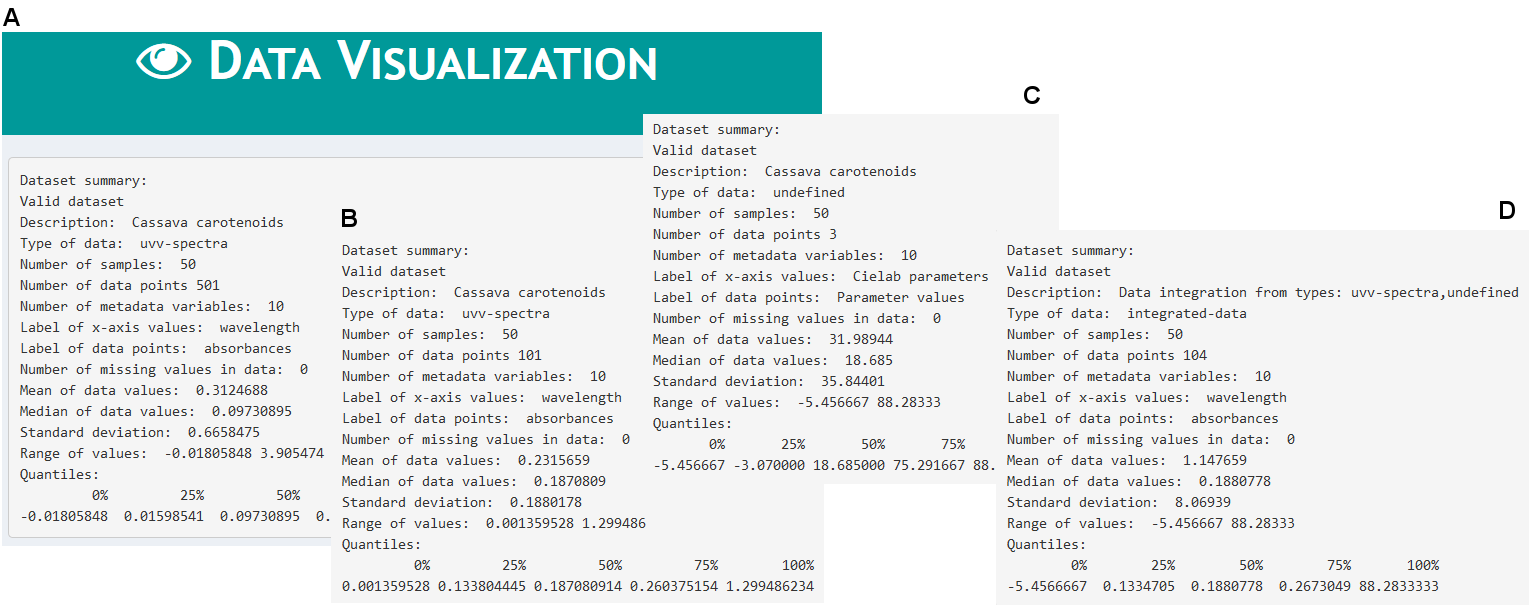
\includegraphics[width=1\linewidth]{Imagens/Case_study/summary_subset_full}
	\caption{Summary of the cassava full \gls{uv} dataset (\textbf{A}) and its subset (wavelengths between 400 and 500 $\eta m$) (\textbf{B}), the CIELAB dataset (\textbf{C}) and the fusion dataset (\textbf{D}), as seen in the web platform.}
	\label{cassava_summary}
\end{figure}

This includes the summary of the cassava full \gls{uv} dataset (\autoref{cassava_summary}A) and its subset with wavelengths between 400 and 500 $\eta m$ (\autoref{cassava_summary}B), the CIELAB dataset (\autoref{cassava_summary}C) and the fusion dataset (\autoref{cassava_summary}D). All datasets are valid, having no missing values they are, therefore, ready for analysis.

All R scripts, raw data and additional analysis pipelines reports are available as supplementary material at \href{http://darwin.di.uminho.pt/pacbb2017/cassava-carotenoids/}{http://darwin.di.uminho.pt/pacbb2017/cassava-carotenoids/}, allowing full reproducibility of the experiments.


\section{Results and Discussion}  \label{results}

\subsection{Determination of carotenoid contents} \label{color_content_subsec}

The \gls{uv} spectrophotometric profiles measured between 200-700 $\eta m$ clearly allow us to discriminate samples according to their carotenoid content. This is more noticeable when comparing the typical \gls{uv} spectrophotometric profiles of cassava samples 5, 23 and 74 (\autoref{UV_spectra}). 


\begin{figure}[h]
	\centering
	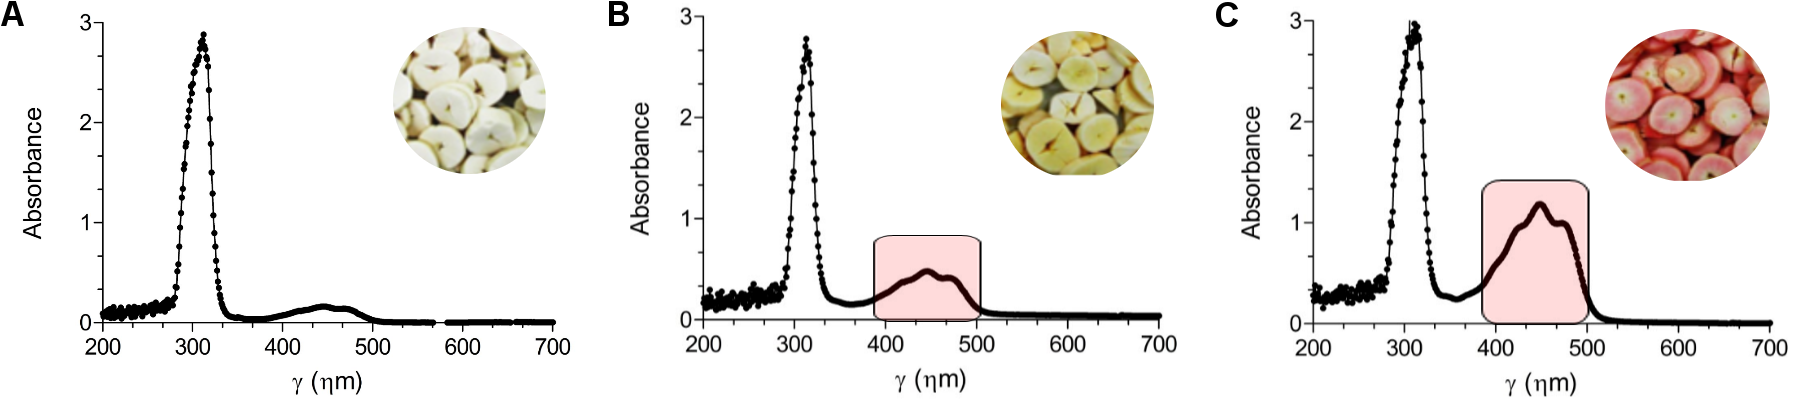
\includegraphics[width=1\linewidth]{Imagens/Case_study/UV_spectra_2}
	\caption{Typical \gls{uv} spectrophotometric profiles ($ \lambda $ = 200-700 $\eta m$, acetone: petroleum ether (v/v)) of root parenchymal tissues of three cassava samples: \textbf{A} - sample 5, \textbf{B} - sample 23 and \textbf{C} - sample 74. The 400-500$\eta m$ region of the spectrum is highlighted in cases \textbf{B} and \textbf{C}.}
	\label{UV_spectra}
\end{figure}

These three samples vary greatly in color, with sample 5 having a cream color, sample 23 a yellow one and the sample 74 a reddish color. In fact, the spectrophotometric profiles differ from each other only at 400-500$\eta m$ region of the spectrum, which is the region where carotenoids typically show absorbance peaks. 

The cream colored sample profile (\autoref{UV_spectra}A) shows an absence of absorbance peaks between the 400-500$\eta m$ region. On the other hand, the yellow colored sample profile (\autoref{UV_spectra}B) shows more noticeable peaks in this region, while the reddish colored sample (\autoref{UV_spectra}C) presents three peaks of great absorption in this region of the spectrum. It is, therefore, expected that the more colored the root the higher carotenoid content it possesses.

On the web platform, the same \gls{uv} spectrophotometric profiles for each sample could be observed in the \textit{Data Visualization} page, with many plot customization options (\autoref{cassava_spectra_plot}).


\begin{figure}[H]
	\centering
	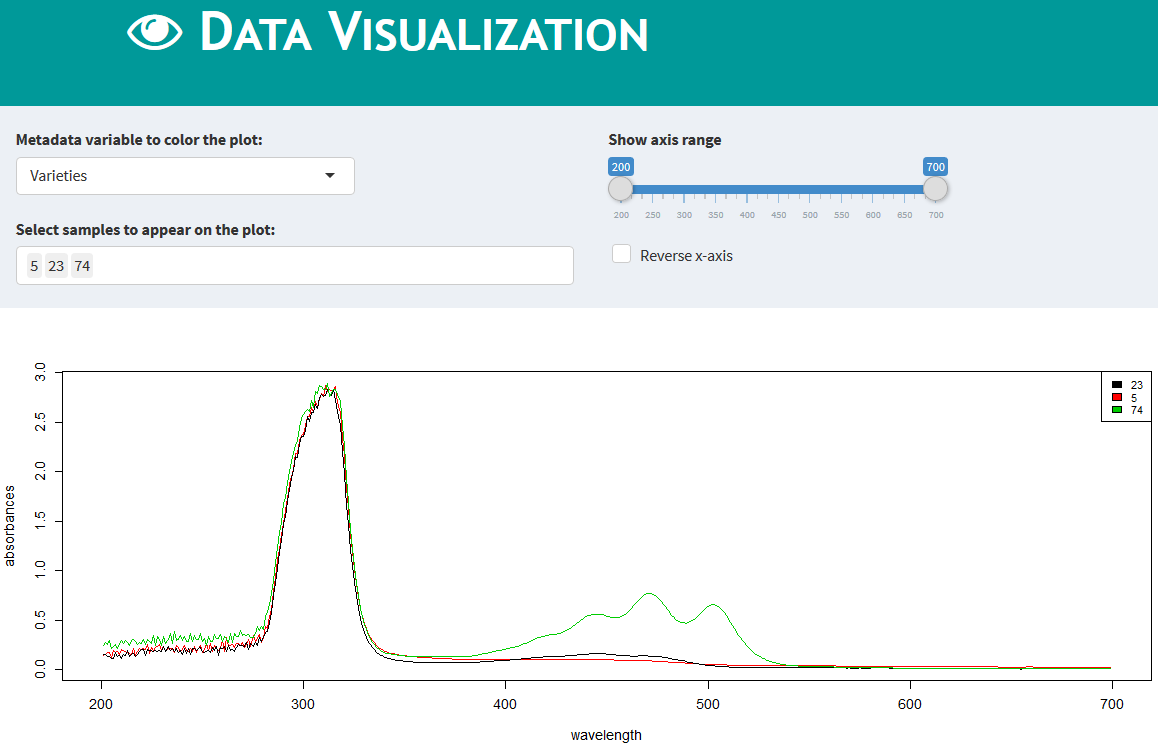
\includegraphics[width=0.8\linewidth]{Imagens/Case_study/spectra_plot}
	\caption{The \gls{uv} spectrophotometric profiles (200 to 700 $\eta m$) of cassava root sample 5 (red), sample 23 (black) and sample 74 (green), as seen on the web platform.}
	\label{cassava_spectra_plot}
\end{figure}


To confirm the possibility of the root color being correlated with its carotenoid contents, the \gls{tcc} was determined by \gls{uv} spectrophotometry, using the Lambert-Beer formula, and is shown in \autoref{carot_content_uv} for each of the fifty fresh root samples.

\begin{figure}[h]
	\centering
	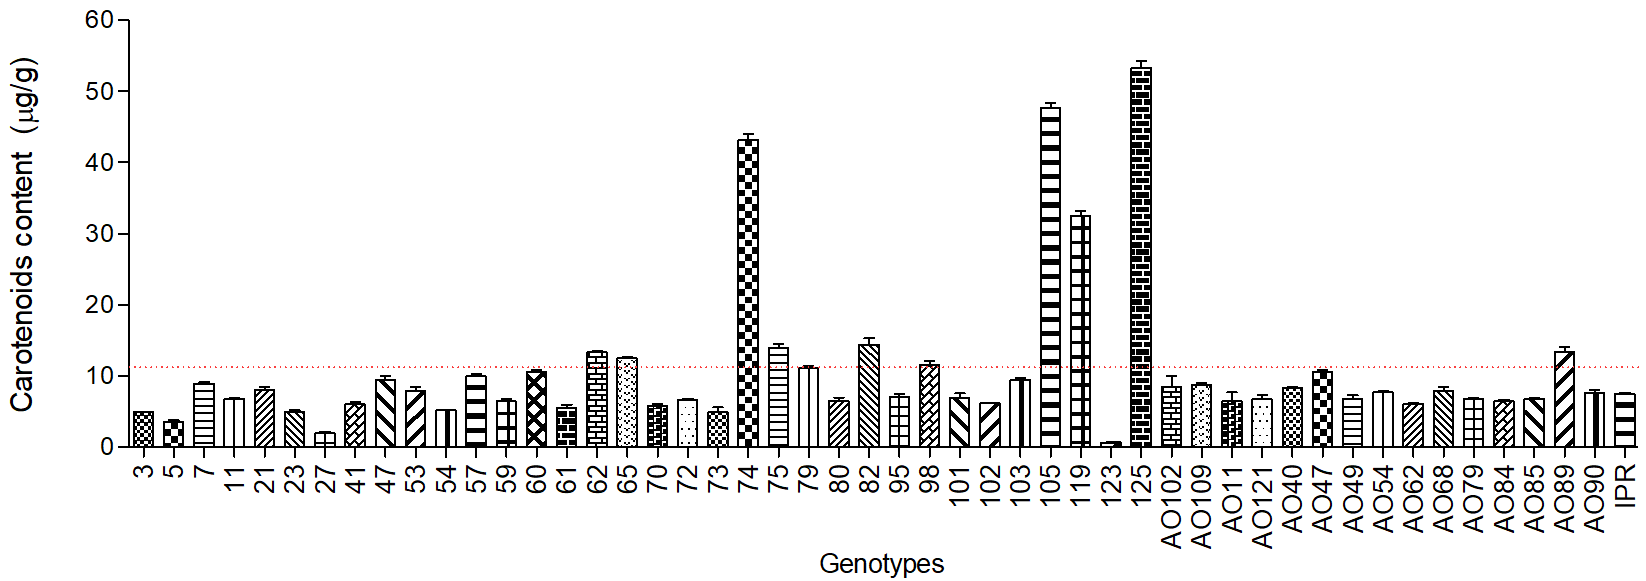
\includegraphics[width=1\linewidth]{Imagens/Case_study/carot_content_uv}
	\caption{Concentration of total carotenoids ($\mu g.g^{-1}$ dry weight $\pm$ standard deviation) in samples of roots of fifty \textit{M. esculenta} genotypes, determined by \gls{uv} spectrophotometry (450 $\eta m$, $\varepsilon$ = 2592 $M^{-1} cm^{-1}$).}
	\label{carot_content_uv}
\end{figure}

A wide disparity in the carotenoid contents is observable, revealing the chemical variability among the analyzed genotypes. In the present study, the cream-colored roots showed the lowest concentrations of total carotenoids, with values around 0.57 $\mu g.g^{-1}$, while higher concentration values were measured in yellow and reddish pigmented roots i.e, 54.93 $\mu g.g^{-1}$. The most abundant carotenoids, trans-$\beta$-carotene and cis-$\beta$-carotene, had concentration values that ranged from 1.82 to 42.82 $\mu g.g^{-1}$ and from 1.19 to 28.86 $\mu g.g^{-1}$, respectively. The results from the \gls{hplc} carotenoid quantification are available in the metadata file.

These findings altogether are consistent with data reported in the literature that observe a positive correlation between the color of the root pulp and the total carotenoid content \citep{champagne2010carotenoid, chavez2005variation, iglesias1997genetic}.


\subsection{CIELAB color space interpretation} \label{cielab_subsec}

To better understand the correlation between samples and the different types of carotenoids with the CIELAB color space, the observed values of L*, a* and b* for each root sample were projected into the CIELAB plane \citep{kljak2014reflectance}. 
The visual interpretation of \autoref{cielab_plot}, showing samples location according to the color of roots in the CIELAB color space, is already sufficient to verify which samples possess higher carotenoid amounts.


\begin{figure}[h]
	\centering
	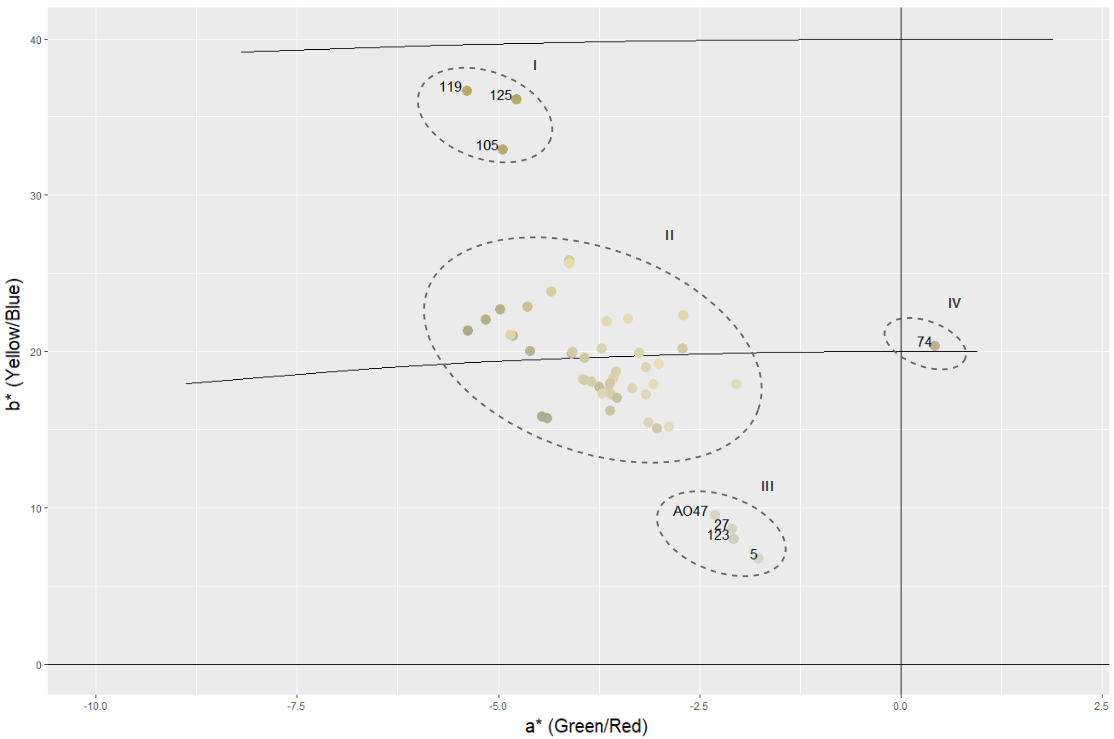
\includegraphics[width=0.7\linewidth]{Imagens/Case_study/cielab_plot2}
	\caption{Location of the cassava samples in the CIELAB color space according to their root pulp colors. The a* value characterizes the coloration in the regions of red (+a*) to green (-a*). The value b* indicates coloring in the range of yellow (+b*) to blue (-b*). Sample identifiers in ellipse II were omitted for easier interpretation of the plot.}
	\label{cielab_plot}
\end{figure}


Samples 105, 119 and 125 (\autoref{cielab_plot}, ellipse I) show high b* values, which stands for the coloration in the yellow range, and these are in fact the samples with the highest carotenoid contents, as it can be observed in \autoref{carot_content_uv}. Interestingly, sample 74 (\autoref{cielab_plot}, ellipse IV) is deviated into the positive axis of a*, which corresponds to the red coloration. In fact, this sample is a reddish root, mostly due to its lycopene content, which confers reddish coloration to the biomass \citep{melendez2007relationship}. It is one of the samples with the highest carotenoid concentration (\autoref{carot_content_uv}).

Samples 123, 27, 05, and AO47 (\autoref{cielab_plot}, ellipse III) were grouped in values of b* closer to zero, these being the samples with the lowest carotenoid content (\autoref{carot_content_uv}). The remaining samples had medium and more similar carotenoid content, being grouped together in a* negative and b* positive values (\autoref{cielab_plot}, ellipse II).


\subsection{Principal Components Analysis} 

The similarity patterns of carotenoid composition found in the previous section were also present among the evaluated genotypes through a \gls{pca} (\autoref{pca_plot}). Information regarding this method is available in \autoref{unsupervised}. 

\begin{figure}[h]
	\centering
	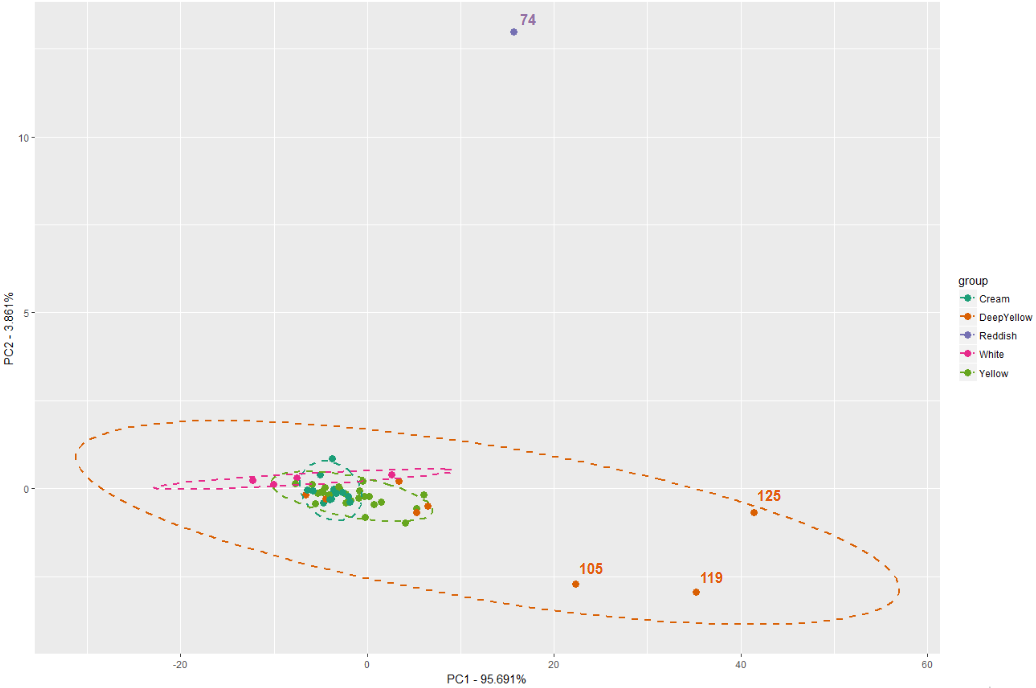
\includegraphics[width=0.7\linewidth]{Imagens/Case_study/pca_plot_3}
	\caption{Scores plot with the distribution of the fifty samples on the first and second \gls{pca} components resulting from the \gls{uv} spectrophotometric data (400-500 $\eta m$), as seen on the web platform. To facilitate the interpretation of the plot, only the sample identifiers for the most relevant samples are shown.}
	\label{pca_plot}
\end{figure}


In their set, PC1 and PC2 explain about 99.5\% of the total variance of the sample population data under this study. The performed \gls{pca} resulted in genotype grouping according to the root pulp coloration, as well as carotenoid quantification, with samples 74, 105, 119, and 125 being the most discrepant within this sample universe \autoref{pca_plot}. 

These being the samples with the highest carotenoid content show that the results here obtained are in accordance with the findings in \autoref{color_content_subsec} that positively correlate the carotenoid content with the color of the cassava roots.


\section{Univariate Analysis} \label{univ_analysis}

To detect significant statistical differences (p-value below 0.05) derived from the effects of cassava's root colors on the spectral profiles a one-way \gls{anova} with Tukey's \gls{hsd} analysis was performed for all wavelengths (200 to 700 $\eta m$). More information about these methods is available in \autoref{univariate}.

For this, the discrete \textit{colors} metadata variable was used, containing the visually determined color of the roots (5 levels:  \textit{Cream}, \textit{DeepYellow}, \textit{Reddish}, \textit{White} and \textit{Yellow}). \autoref{cassava_anova}A shows the top ten results ordered by decreasing p-value. In \autoref{cassava_anova}B the -log$_{10}$ of p-values plot is represented, showing an horizontal line that corresponds to a p-value threshold of 0.05. 

\begin{figure}[h]
	\centering
	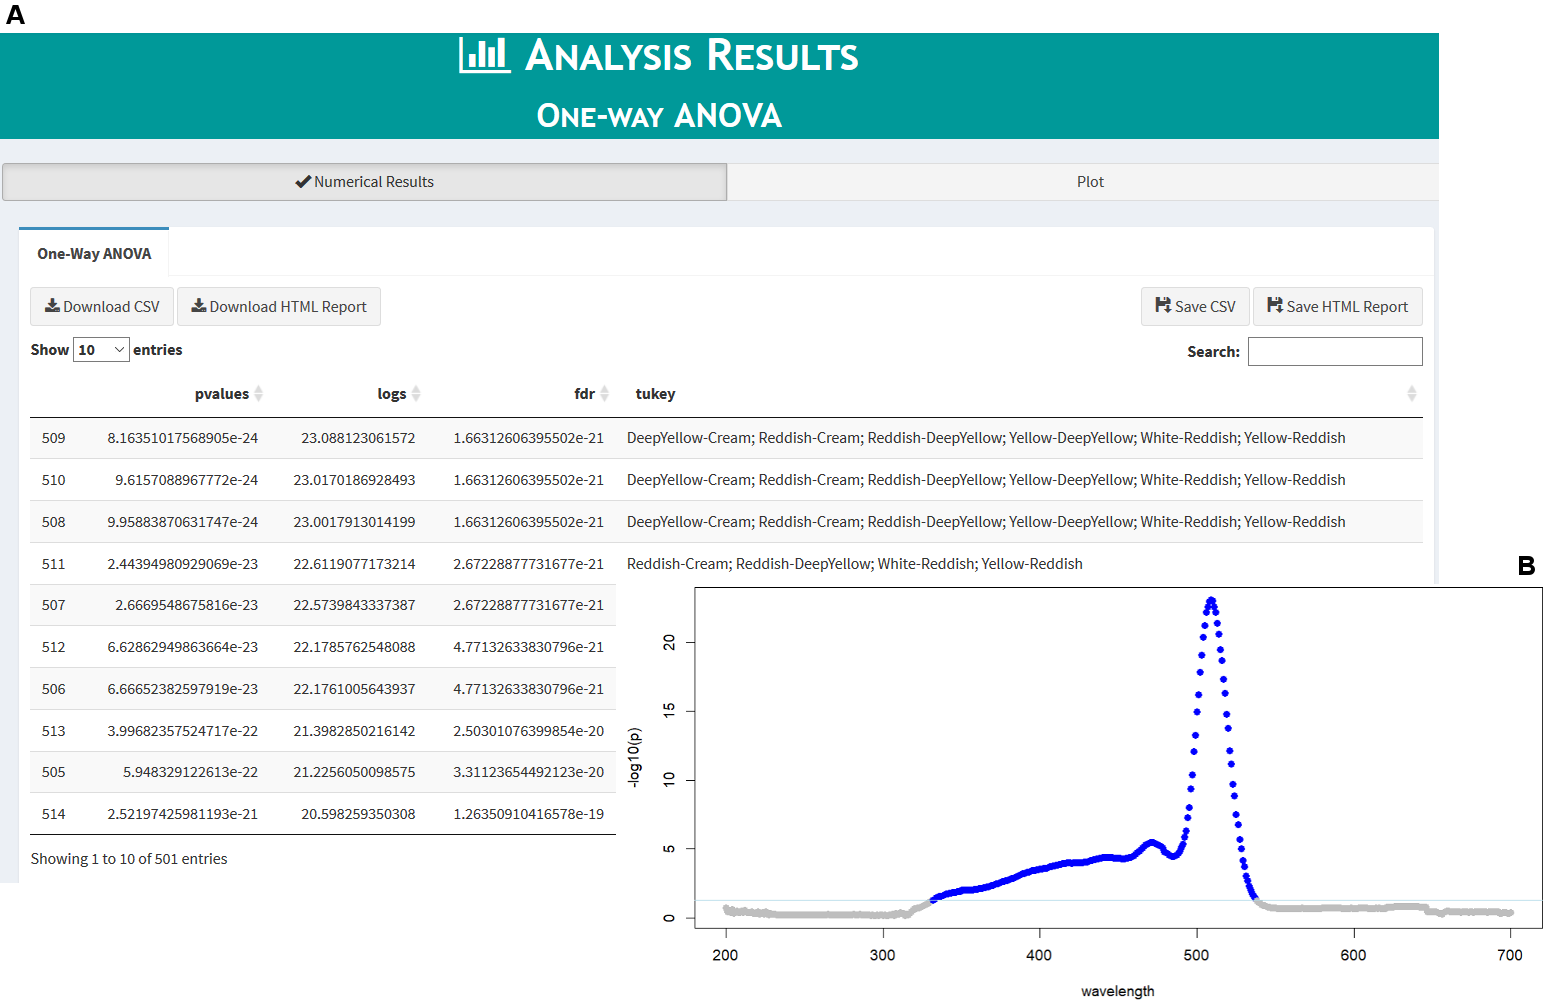
\includegraphics[width=1\linewidth]{Imagens/Case_study/anova_table_plot}
	\caption{\gls{anova} results using the discrete \textit{colors} metadata variable (\textbf{A}) and respective plot of the -log$_{10}$ of p-values with a p-value threshold value of 0.05 (\textbf{B}), as seen on the web platform.}
	\label{cassava_anova}
\end{figure}

From \autoref{cassava_anova} it appears that wavelengths around 500$\eta m$ have a significant effect on the discrimination of cassava samples according to their color. This finding becomes more evident when looking at the -log$_{10}$ of p-values plot.


\section{Machine Learning}

\subsection{Carotenoid content prediction using \gls{uv} data} \label{ml_uv_subsec}

In \autoref{UV_table}, the performance values obtained with the various machine learning models using \gls{uv} data (400-500 $\eta m$) as input and the \gls{tcc} determined by spectrophotometry (Lambert-Beer formula), the \gls{tcc} determined by \gls{hplc} and the total content of trans-$\beta$-carotene (the most abundant carotene in cassava roots) as response prediction variables are shown.


\begin{table}[h]
	\centering
	\caption{Performance values (\gls{rmse} and $R^{2}$) obtained for the different machine learning models trained with \gls{uv} spectrophotometry data (400-500 $\eta m$). The \acrfull{tcc} determined by spectrophotometry (Lambert-Beer formula), the \gls{tcc} determined by \gls{hplc} and the total content of trans-$\beta$-carotene (the most abundant carotene in cassava roots) were used as response prediction variables. The parenthesis indicate the package specific method chosen for the simulation, with exception to the linear regression models.}	
	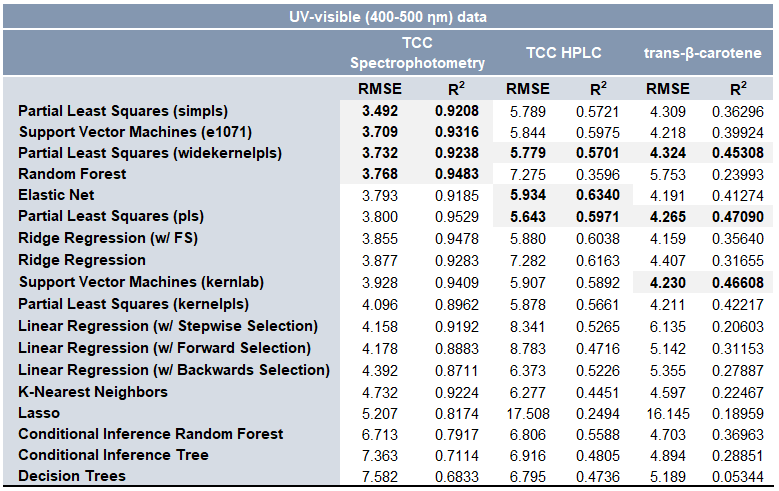
\includegraphics[width=1\linewidth]{Imagens/Case_study/UV_table}
	\label{UV_table}
\end{table}


The highest $R^{2}$ performance values (above 90\%) and lowest \gls{rmse} values were obtained when using the \gls{tcc} determined using spectrophotometric data as response variable. This was expected considering that both input and response data used employ the same physical phenomenon of detection of compounds (absorbance). The models that best performed in this case were \gls{pls} using both \textit{simpls} and \textit{widekernelpls} methods, \gls{svm}s and random forests with \gls{rmse} performance values of 3.492, 3.732, 3.709 and 3.768, respectively.

Using the \gls{tcc} determined by \gls{hplc} as the response variable, a small decrease in performance values is observed, with \gls{pls} (\textit{widekernelpls} and \textit{pls} methods) and elastic network showing best performance with \gls{rmse} values of 5.779, 5.643 and 5.934, respectively, and $R^{2}$ values around 60\%.

The worst results were obtained when using trans-$\beta$-carotene as response variable, with best performance models being \gls{pls} (\textit{widekernelpls} and \textit{pls} methods) and \gls{svm}s, with \gls{rmse} values of 4.324, 4.265 and 4.230, respectively, and $R^{2}$ values around 46\%.

When observed, the values of \acrfull{vip} for this analysis (supplementary material), which identify the most relevant variables for the validation of the method, it can be detected that the wavelengths 449, 448 and 450 nm (precisely the wavelength that is used for the quantification of $\beta$-carotene through the Lambert-Beer formula) were used in 100\%, 99.93\% and 99.76\% of cross-validation training performance. This result is important in the sense that it attests to the robustness of the models in predicting the contents of these compounds in cassava samples.

By pre-processing the data, as well as applying feature selection, an overall increase in model performance for most models used was observed (supplementary material). In \autoref{UV_preproc_table} one such case is shown, where using pre-processed \gls{uv} data as input to Random Forest model (best performing model with raw data) increased even further model performance. By applying smoothing interpolation, background and offset corrections, or background correction alone, \gls{rmse} values decreased from 6.194 to 5.773, 5.936 and 6.175, respectively. $R^{2}$ values also increased from 55\% to around 60\% in each case.


\begin{table}[h]
	\centering
	\caption{Performance values (\gls{rmse} and $R^{2}$) obtained for a random forest model trained with \gls{uv} spectrophotometry data (400-500 $\eta m$), applying several pre-processing methods to the data. The \gls{tcc} determined by \gls{hplc} was used as response prediction variable.}	
	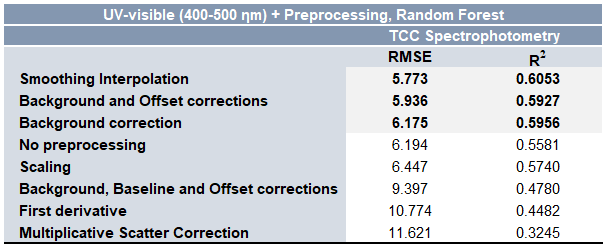
\includegraphics[width=0.8\linewidth]{Imagens/Case_study/UV_preproc_table}
	\label{UV_preproc_table}	
\end{table}


\subsection{Carotenoid content prediction using CIELAB data} \label{ml_cielab_subsec}

The performance values obtained by using CIELAB data as input to the various machine learning models are shown in \autoref{CIELAB_table}. The \gls{tcc} determined by spectrophotometry (Lambert-Beer formula), the \gls{tcc} determined by \gls{hplc} and the total content of trans-$\beta$-carotene (the most abundant carotene in cassava roots) were used as response prediction variables.


\begin{table}[h]
	\centering
	\caption{Performance values (\gls{rmse} and $R^{2}$) obtained for the different machine learning models trained with CIELAB data. The \gls{tcc} determined by spectrophotometry (Lambert-Beer formula), the \gls{tcc} determined by \gls{hplc} and the total content of trans-$\beta$-carotene (the most abundant carotene in cassava roots) were used as response prediction variables. The parenthesis indicate the package specific method chosen for the simulation.}	
	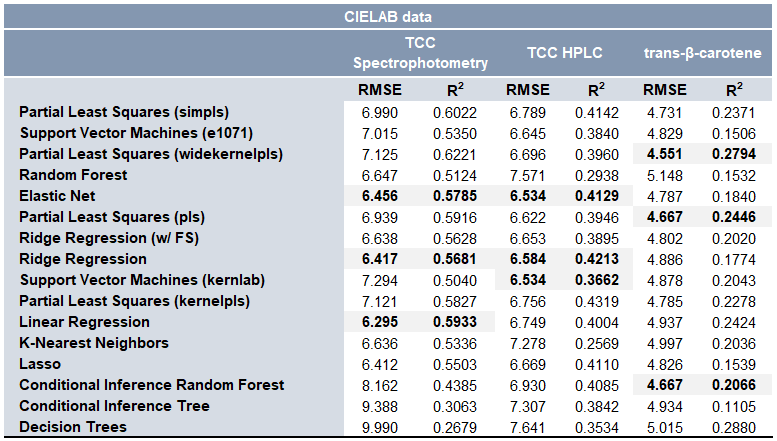
\includegraphics[width=1\linewidth]{Imagens/Case_study/CIELAB_table}
	\label{CIELAB_table}	
\end{table}


Similarly to the results obtained in \autoref{ml_uv_subsec}, highest $R^{2}$ performance values and lowest \gls{rmse} values were obtained when using the \gls{tcc} determined using spectrophotometric data as a response prediction variable. There is, however, a noticeable overall decrease in model performance when using all three prediction variables. This is easily explained by the number of features present in the data, considering that in this case only three features are present (L*, a* and b*), while in the previous case there were far more features, about 101 (data measured from 400 to 500$\eta m$).

Using the \gls{tcc} determined by spectrophotometry as response variable, the models that showed best performance were linear and ridge regressions and elastic network with \gls{rmse} values of 6.295, 6.417 and 6.456, respectively, with $R^{2}$ values around 60\%. 

For the second variable, \gls{tcc} determined by \gls{hplc}, the best models were elastic network, ridge regression and \gls{svm}s with \gls{rmse} values of 6.534, 6.584 and 6.534, respectively, and $R^{2}$ values around 40\%. 

Lower \gls{rmse} values were observed when using trans-$\beta$-carotene as response variable, with best performance models being \gls{pls} (\textit{widekernelpls} and \textit{pls} methods) and conditional inference random forests, with \gls{rmse} values of 4.551, 4.667 and 4.667, respectively. However, models showed a decrease in the fitting of the data with an $R^{2}$ around 25\%.

Looking at the \gls{vip} (supplementary material), the variables that played the most important role in the prediction of carotenoid content in the cassava samples are evident. The b* parameter was relevant about 100\% of the cases, which was somewhat expected, considering that the samples are widely distributed across the \textit{y} axis in \autoref{cielab_plot}, which corresponds to the b* parameter. Looking at the same plot we can see that the a* interval in which samples are distributed is not as wide, however, this parameter was relevant in about 56\% of the predictions. With a VIP of 0\% the L* parameter was the least relevant of the three.

The only pre-processing method applied to CIELAB data was scaling, as the other methods would not make much sense considering they are aimed at spectral data. Applying the scaling to the data showed an increase in model performance, however limited (supplementary material).



\subsection{Carotenoid content prediction using fusion data} \label{ml_fusion_subsec}

The performance values obtained by using a \gls{llf} between \gls{uv} (400-500 $\eta m$) and CIELAB data as input to the various machine learning models are shown in \autoref{UV_cielab_table}. Similarly to the previous cases, the response prediction variables used were the \gls{tcc} determined by spectrophotometry (Lambert-Beer formula), the \gls{tcc} determined by \gls{hplc} and the total content of trans-$\beta$-carotene.


\begin{table}[h]
	\centering
	\caption{Performance values (\gls{rmse} and $R^{2}$) obtained for the different machine learning models trained with a fusion between \gls{uv} spectrophotometry and CIELAB data. The \gls{tcc} determined by spectrophotometry (Lambert-Beer formula), the \gls{tcc} determined by \gls{hplc} and the total content of trans-$\beta$-carotene (the most abundant carotene in cassava roots) were used as response prediction variables. The parenthesis indicate the package specific method chosen for the simulation, with exception to the linear regression models.}	
	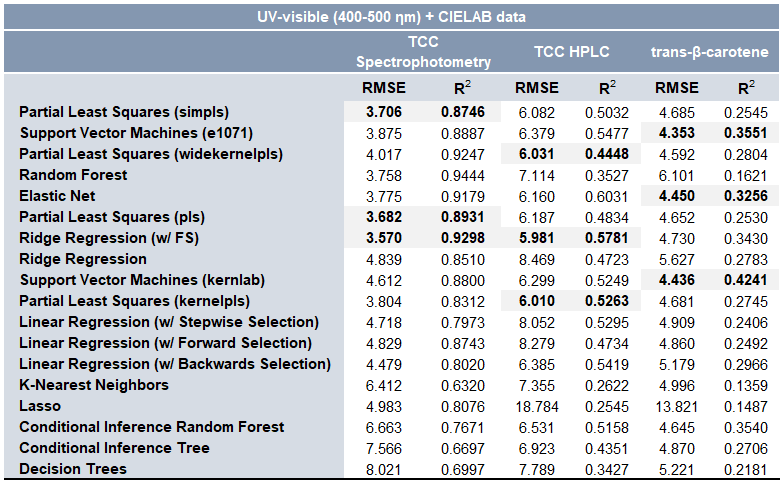
\includegraphics[width=1\linewidth]{Imagens/Case_study/UV_cielab_table}
	\label{UV_cielab_table}	
\end{table}


The results obtained for fusion data are similar to those in \autoref{ml_uv_subsec} and \autoref{ml_cielab_subsec} in the sense that highest $R^{2}$ performance values and lowest \gls{rmse} values were obtained when using the \gls{tcc} determined using spectrophotometric data as response prediction variable. Overall there is an increase in model performance when comparing to the results obtained for \gls{uv} data alone.

The best model performance when using the \gls{tcc} determined by spectrophotometry as response variable was achieved by ridge regression (with feature selection) and \gls{pls} (\textit{pls} and \textit{simpls} methods) models with \gls{rmse} values of 3.570, 3.682 and 3.706, respectively, and $R^{2}$ values around 90\%.

For the variable \gls{tcc} determined by \gls{hplc}, the models that best performed were ridge regression (with feature selection) and \gls{pls} (\textit{kernelpls} and \textit{widekernelpls}) models, having \gls{rmse} values of 5.981, 6.010 and 6.031, respectively, with $R^{2}$ values around 50\%.

Similarly to the previous cases, lower \gls{rmse} values were observed when using trans-$\beta$-carotene as prediction variable, with best performance models being SVMs (\textit{e1071} and \textit{kernlab} methods) and elastic network with \gls{rmse} values of 4.353, 4.436 and 4.450, respectively, and $R^{2}$ values around 30\%.

The \gls{vip} computed for this case (supplementary material) showed that the variables which presented the most important role in the prediction of carotenoid content in the cassava samples were those of wavelength around 170$\eta m$ (VIPs $>$ 99\%). Here, the CIELAB b* parameter was relevant in about 65\% of predictions, while the a* and L* parameters had a VIP close to zero.

The only preprocessing method applied to the fusion data was scaling, as the methods employed in \autoref{ml_uv_subsec} are aimed at spectral data. Data filtering was also applied to the data. Both methods contributed to an overall increase in model performance when compared to the performance obtained using raw \gls{uv} data (supplementary material).


\section{Conclusions} \label{conclusions}

The present study has shown how CIELAB color measurement can be used as a fast and non-destructive method to calibrate for the total carotenoid content of cassava genotypes roots with acceptable prediction error. The  \gls{llf} of \gls{uv} spectrophotometry and CIELAB data has demonstrated how data fusion can lead to a better model performance for prediction when comparing to the use of a single data source, having similar results been found in the literature \citep{botwey2014multi}.

Furthermore, the \gls{uv} spectrophotometric profiles measured between 400-500$\eta m$ and the consequent carotenoid content determination allowed the observation of a positive correlation between the color of the root pulp and the \gls{tcc}, which is in accordance with data reported in the literature \citep{champagne2010carotenoid, chavez2005variation, iglesias1997genetic}. This finding was more explicit when observing the projection of the fifty cassava root samples in the CIELAB color space plane, having several clusters been formed, where the highest values of b* (which stands for the yellow coloration) and a* (which stands for the red coloration) were associated to the samples with highest carotenoid contents.

Additionally, the information obtained by coupling the analysis of pro-vitamin A biochemical markers to bioinformatics tools helps supporting the rational design of biochemically-assisted breeding programs of \textit{M. esculenta}, that aim to obtain cultivars with high levels of pro-vitamin A carotenoids and superior nutritional traits.














